\chapter{New middleware architecture}

\section{Design goals and core concepts}

\section{Architecture overview}

The PerLa Middleware is responsible for managing the lifecycle of all devices
connected to the PerLa framework, and for providing a uniform API to interact
with them. Its design revolves around the Functionality Proxy Component
(\texttt{FPC}), a self-contained proxy object that embeds all the logic
required to communicate with a single remote device.  The most prominent trait
of the \texttt{FPC} is its interface, an API that allows PerLa users to
interact with the sensing network through two hardware-agnostic communication
primitives, named get() and set().  Use of this interface neither requires
knowledge of the sensing network, nor of the device that will ultimately
perform the requested operation.

\begin{figure}[h!]
\center
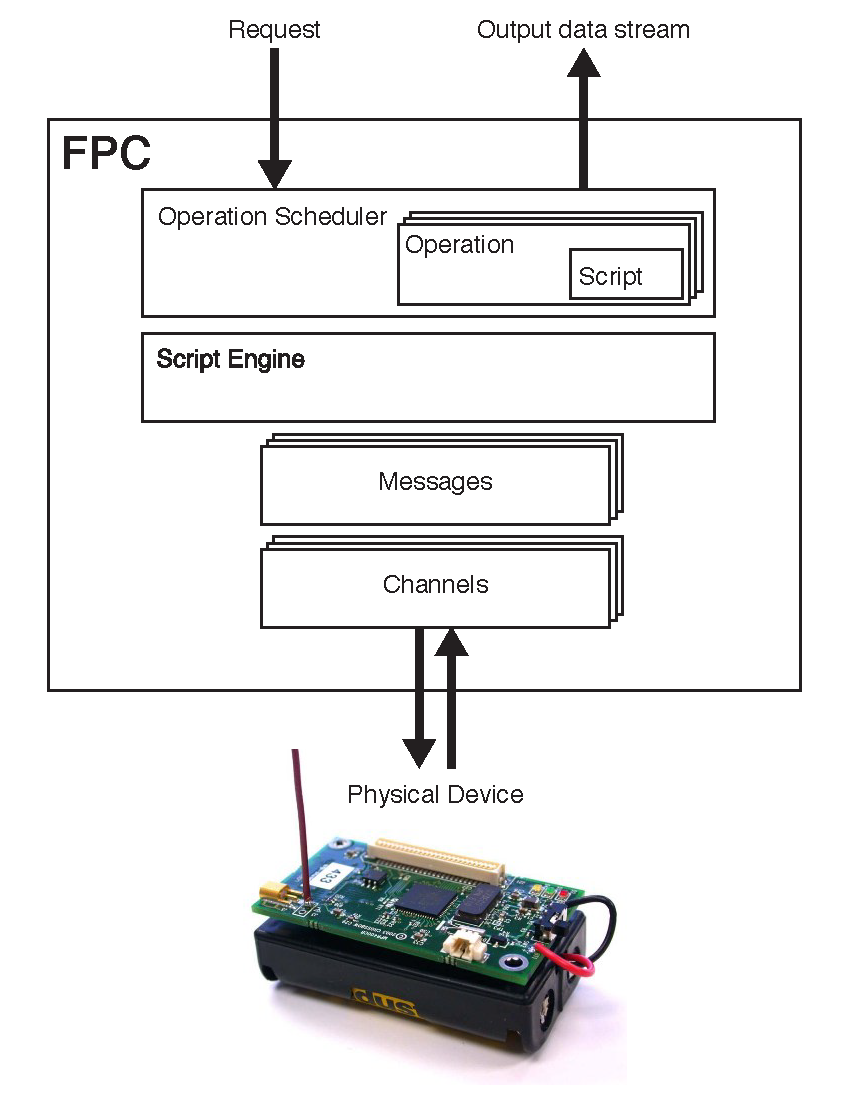
\includegraphics[width=0.6\textwidth]{imgs/fpc.pdf}
\caption{Internal FPC structure}
\label{fig:fpc_overview}
\end{figure}

Each \texttt{FPC} is formed from the composition of various independent
software units, each of which is responsible for the management of a single
aspect of the interaction with the remote device (see
figure~\ref{fig:fpc_overview}). This modular design was chosen to promote
reusability and foster future expandability through composition of
independent objects. The following list contains a synopsis of the modules
that form an \texttt{FPC}:

\begin{itemize}

    \item \textbf{Channel:} A software component capable of performing I/O
    operations. \texttt{Channels} are responsible for managing the
    communication between the PerLa framework and the remote devices;

    \item \textbf{Mapper:} A data marshaller/unmarshaller. \texttt{Mappers}
    allow the \texttt{FPC} to interpret byte streams received from a Channel,
    and to serialize high-level data structures prior to transmission;

    \item \textbf{Script Engine:} An interpreter for executing PerLa
    \texttt{Scripts}, small programs written in a proprietary PerLa scripting
    language, which are used to dynamically bind high level data requests to
    native processing tasks performed on the remote device;

    \item \textbf{Operation Scheduler:} Schedules the execution of concurrent
    data collection operations on the remote device. The scheduler may simulate
    certain operations if the device connected to the FPC is not able to
    perform them natively (e.g., periodic sampling may be simulated by polling
    the remote device at regular intervals).

\end{itemize}

New \texttt{FPC} objects are instantiated at runtime by the
\texttt{FPCFactory}. The starting point for the creation of an \texttt{FPC} is
the Device Descriptor, an XML document which contains a machine parseable
description of a single sensing device. Device Descriptors are organised in
different sections, each of which defines the configuration of one of the
aforementioned \texttt{FPC} modules. The \texttt{FPCFactory} can receive new
Device Descriptors directly from the node being connected (Plug\&Play
behaviour), or from another entity that acts on behalf of it (off-band
behaviour). The latter approach allows devices which are not capable of
autonomously transmit their Device Descriptor to be registered on the PerLa
Middleware.

\begin{figure}[h!]
\label{fig:fpc_overview}
\includegraphics[width=\textwidth]{imgs/middleware_overview.pdf}
\caption{Internal FPC structure}
\end{figure}

A reference to each \texttt{FPC} is stored in the \texttt{Registry}, a
Middleware component that is responsible for maintaining a complete index of
all devices accessible through the PerLa framework. Thanks to the
\texttt{Registry}, PerLa user can discover sensing nodes through
capability-based queries, and retrieve the \texttt{FPC} objects that can be
used to interact with them.

\subsection{Asynchronous interaction paradigm}
\label{sec:newmiddleware.async}

One of the major differences between the New and Classic Middleware
architectures lies in the paradigm employed to interconnect all internal
modules of the PerLa software infrastructure. The New Middleware design
introduces a fully asynchronous interaction paradigm that deviates profoundly
from the mechanism previously promoted, as it is based on the idea of
thread-less module composition.

Within the previous Middleware architecture, a connection between two different
modules was achieved by means of a decoupling element dubbed \texttt{Pipe}, a
one-way message queue designed to shuttle data elements from a software
component to its intended receiver. This system proved to be crucial in the
first development stages of PerLa, as its generic interface allowed the early
designers to experiment with several competing architectures and component
combinations. However, its flexibility came at a cost, both in terms of
performances and API readability. First of all, each \texttt{Pipe} allocated an
initial memory cache of 10 data elements. Moreover, the receiving end of a
\texttt{Pipe}, namely the \texttt{Waiter}, was required to instantiate a Java
thread dedicated solely to the reception of data messages. The widespread use
of the \texttt{Pipe}-\texttt{Waiter} paradigm thus led to the proliferation of
threads and to an overuse of memory, which negatively impacted the overall
system efficiency. In addition, the loosely coupled interaction paradigm
promoted by the Classic Middleware resulted in a weak API that lacked semantic
clarity.

The new 

Although this may not seem as an advantage, as long-running operations must be
performed in a thread nonetheless, short activities



\subsection{Factory patterns}
\label{sec:newmiddleware.factory}

\subsection{Device Descriptor and Plugin system}
\label{sec:newmiddleware.descriptor}
